%% Sifter paper -- Research Synthesis Methods, article type Software Focus.
%% Class: CUP-JNL-DTM with journal=rsm (biblatex, NEJM-ish numbered superscript).
%% Build: make (pdflatex -> biber -> pdflatex x2)
\documentclass[journal=rsm]{CUP-JNL-DTM}

\usepackage{graphicx}
\usepackage{amsmath,amssymb}
\usepackage[T1]{fontenc}
\usepackage[colorlinks,allcolors=blue]{hyperref}
\usepackage{tikz}
\usetikzlibrary{arrows.meta,positioning,shapes.geometric}
\usepackage{xcolor}

\graphicspath{{figures/}}

\jname{Research Synthesis Methods}
\articletype{Software Focus}
\jyear{2026}

\addbibresource{references.bib}

\begin{document}

\begin{Frontmatter}

\title[Sifter: LLM-assisted screening for systematic reviews]{Sifter: an open-source, provider-agnostic platform for large language model assisted screening in systematic reviews}

\author[1]{Fabricio G. Scaglioni}
%% TODO coautores: orientadores (Marilton Aguiar e Julius Leite, UFPel) e demais
%% colaboradores entram aqui com \author[1]{} e a ordem acordada com eles.

\authormark{Scaglioni}

\address[1]{\orgdiv{Programa de P\'os-Gradua\c{c}\~ao em Computa\c{c}\~ao}, \orgname{Universidade Federal de Pelotas}, \orgaddress{\city{Pelotas}, \state{RS}, \country{Brazil}}. \email{fabricio.scaglioni@ufpel.edu.br}}

\keywords{systematic reviews, screening, large language models, automation, reproducibility}

\abstract{Title and abstract screening is the most labour-intensive step of a
systematic review, and the step where automation has been slowest to become
trustworthy. Sifter is an open-source platform that delegates screening to
large language models (LLMs) while keeping the review protocol, the decision
trail and the cost accounting under the reviewer's control. The platform is
provider-agnostic, stores one structured decision per record (include,
exclude or doubt) together with a short justification, and offers a blind
validation mode in which the model decision is hidden until the human
reviewer records their own, from which agreement statistics are computed
automatically. In a pilot deployment across four review projects, 14{,}219 of
14{,}353 records (99.1\%) received an LLM decision at an average of 833 tokens
per record, which corresponds to US\$0.10 to US\$1.63 per 1{,}000 screened
records depending on the provider tariff. On an educational corpus of 31
blindly re-screened records, agreement with the human reviewer was substantial
(Cohen's $\kappa$ 0.61, 95\% CI 0.29 to 0.90) with no missed inclusion
(sensitivity 100\%, specificity 80\%). We describe the design decisions that
make these numbers auditable, report the platform against current expectations
for generative AI in evidence synthesis, and state precisely which workload
metrics remain to be measured before the tool can be recommended for
production use.}

\end{Frontmatter}

\section*{Highlights}

\begin{itemize}
\item Sifter is a web-based, open-source platform that lets a review team run
title and abstract screening with large language models without giving up
control of the protocol, the audit trail or the cost.
\item Every automated decision is stored with the record, the model, the prompt
version and the token counts, so a reviewer can reconstruct what happened to
any single study months later.
\item A blind validation mode hides the model decision until a human has
screened the same record, which turns routine re-screening into a measurable
agreement study instead of an unverifiable claim of accuracy.
\item In a pilot deployment the marginal cost of screening was between US\$0.10
and US\$1.63 per thousand records, small against the reviewer hours it
displaces; the open question is not cost but the rate of missed inclusions,
which the platform is designed to expose rather than hide.

\end{itemize}

\section{Introduction}\label{sec:intro}

A systematic review begins with a search that returns thousands of records, and
every one of them has to be judged against pre-specified eligibility criteria
before a single study is read in full. This title and abstract screening stage
is consistently reported as the most time-consuming part of the review
process, and it is the stage where reviewer fatigue translates most directly
into inconsistent decisions \autocite{Tsafnat_2014}. The methodological
response has been to accept some degree of automation provided that the
automation is itself evaluated: the question is no longer whether machine
decisions may assist screening, but how their errors are measured and
reported.

Two families of tools have addressed the problem. Workflow systems such as
Rayyan, Covidence, DistillerSR and EPPI-Reviewer organise the screening work
but leave the judgement to the reviewer
\autocite{Ouzzani_2016,Marshall_2019}. Machine learning systems such as
ASReview, SWIFT-Review and the RCT classifiers derived from RobotSearch learn
from a small set of labelled records and then rank the remaining ones, so that
the reviewer reads the most promising records first
\autocite{van_de_Schoot_2021,Howard_2016}. Both families are useful, and both
have a structural limitation for the question this paper addresses: the
workflow systems produce no machine decision to evaluate, and the supervised
systems produce a ranking whose quality depends on the seed labels supplied by
the reviewer, which makes the result difficult to transfer across reviews.

Large language models change the shape of the problem. A general-purpose model
can be given the review protocol in the prompt and return a decision with a
short justification, without any task-specific training data. Early evidence
is encouraging but uneven. Khraisha and colleagues found that GPT-4 could
screen and extract data with performance that varied substantially by task and
by field \autocite{Khraisha_2024}; Gartlehner and colleagues reported a
similar pattern for data extraction \autocite{Gartlehner_2024}. At the same
time, Callaghan and colleagues argued that computer-assisted screening tools
are frequently released without the evaluation needed to justify their use in
evidence synthesis \autocite{Callaghan_2024}, and the journal has since
published explicit reporting expectations for manuscripts that evaluate
generative AI in systematic reviews and meta-analyses
\autocite{Farotimi_2025}.

That combination, promising capability plus a weak evidence base, defines the
gap this paper addresses. What a review team needs is not another model but an
instrument: a system in which the model can be replaced, in which every
automated decision is traceable to a record, a prompt and a model version, in
which cost is accounted per record rather than per project, and in which the
agreement between the model and a human reviewer can be measured on demand
rather than asserted in a paper. The absence of that instrument is, in our
reading, one reason why the literature on LLM screening is dominated by
one-off evaluations on curated datasets and thin on deployments inside real
reviews.

This paper describes \textsc{Sifter}, an open-source platform built to be that
instrument, and reports what a pilot deployment measured. The contribution is
threefold. First, we describe the design decisions that make LLM screening
auditable: a protocol object that is the single source for every prompt, a
three-way decision space in which \emph{doubt} is a first-class outcome
returned to the human reviewer, and a blind validation mode that hides the
model decision until the reviewer has recorded their own. Second, we report
the pilot evaluation: 14{,}219 records screened across four projects, the token
and monetary cost per record, and an agreement study on an educational corpus.
Third, we report the platform against the reporting expectations for
generative AI in evidence synthesis \autocite{Farotimi_2025} and state
explicitly which workload metrics, notably work saved over screening and
number needed to read, have not yet been measured.

The remainder of the paper is organised as follows.
Section~\ref{sec:related} situates the platform among existing review software
and screening automation. Section~\ref{sec:system} describes the architecture
and the screening pipeline. Section~\ref{sec:evaluation} reports the pilot
deployment. Section~\ref{sec:discussion} discusses what the numbers do and do
not establish, and Section~\ref{sec:conclusion} concludes.

\section{Related work}\label{sec:related}

\subsection{Review workflow software}

Rayyan, Covidence, DistillerSR and EPPI-Reviewer share a common design: they
hold the record set, distribute records among reviewers, record include and
exclude decisions, and resolve conflicts
\autocite{Ouzzani_2016,Marshall_2019}. Their contribution is organisational,
and it is substantial: duplicate removal, blind dual screening and conflict
resolution are the mechanisms through which the method protects itself. None
of them, however, produces an automated screening decision that can be
compared with the human one. When a review reports the use of such a tool, the
report describes the workflow, not the performance of an algorithm.

\subsection{Machine learning and active learning}

ASReview introduced an open, actively learned screening loop in which the
reviewer labels records one at a time and the model reorders the remaining
queue after each label \autocite{van_de_Schoot_2021}. SWIFT-Review combined
text mining, clustering and classification in a workbench for scoping
\autocite{Howard_2016}. These systems are evaluated with recall-oriented
metrics, and their reported performance is best understood as the performance
of a prioritisation policy conditioned on the seed labels: change the seeds
and the curve changes. That property is not a defect, but it complicates
transfer, because a review team cannot know in advance what the seed labels
will buy them.

\subsection{Large language models in screening and extraction}

The recent literature moves the decision itself into the model. Khraisha and
colleagues evaluated GPT-4 on screening and data extraction across a set of
reviews and found performance that was usable in some tasks and unreliable in
others \autocite{Khraisha_2024}. Gartlehner and colleagues reached a similar
conclusion for extraction, with a proof-of-concept design
\autocite{Gartlehner_2024}. Reviews of the wider automation landscape stress
that the field lacks shared reporting standards for these evaluations and that
many tools are published without them \autocite{Callaghan_2024}. The journal's
guidance for manuscripts testing generative AI now specifies the minimum:
documented prompts, established metrics, external validation, seeds, model
versions and access dates, and public data and code \autocite{Farotimi_2025}.

\subsection{What is missing}

Three things, in our reading. First, a deployment description: most LLM
screening studies run on a curated benchmark, not inside a review that a team
actually needed to finish. Second, cost accounting at the record level, which
is what determines whether a review of 15{,}000 records is feasible under a
given budget. Third, an instrument that makes the agreement study repeatable:
if computing $\kappa$ between model and reviewer requires a separate script and
a separate dataset, it will be done once, for the paper, and never again. The
platform described next is an attempt to make these three things ordinary.

\section{The Sifter platform}\label{sec:system}

\subsection{Design goals}

Sifter was built for one recurring situation: a review team has a protocol, a
record set of a few thousand items, and a limited number of reviewer hours.
The platform is the result of four requirements that were treated as
non-negotiable, summarised in Table~\ref{tab:goals}. Each of them rules out a
design that would otherwise have been simpler.

\begin{table}[htbp]
\centering
\caption{Design goals and the mechanism that implements each one in Sifter}
\label{tab:goals}
\begin{tabular}{@{}p{0.19\textwidth}p{0.37\textwidth}p{0.27\textwidth}@{}}
\toprule
Goal & Mechanism & Where it is visible \\
\midrule
Auditability &
One decision row per record, carrying label, justification, model identifier,
prompt version and token counts &
Record detail view; CSV and JSON export \\
Provider independence &
A provider abstraction with one generic OpenAI-compatible adapter plus native
adapters for Gemini, Anthropic and Vertex AI &
Project settings; per-project model choice recorded with the decisions \\
Human primacy &
Three-way decision space in which \emph{doubt} is a first-class label, returned
to the reviewer rather than forced into include or exclude &
Queue filter; doubt tab \\
Measured agreement &
Blind validation mode that hides the model decision until the human decision is
stored, then computes $\kappa$, its confidence interval and the confusion
matrix &
Validation dashboard of the project \\
\bottomrule
\end{tabular}
\end{table}

\subsection{Architecture}

Sifter is a three-tier web application. The backend is a FastAPI service with
SQLAlchemy over PostgreSQL; the frontend is a SvelteKit single-page
application; the whole system is distributed as a Docker Compose stack with
four services (application programming interface, database, test database and
frontend), which is also the installation path recommended to reviewers who
want to run the tool locally. Review data are isolated per project: records,
protocol, decisions and events are scoped to a project identifier, and the
storage layer keeps the associated PDFs in a per-project directory.

The architecture is deliberately unremarkable. The parts that matter for
evidence synthesis are not the web framework but the objects the framework
persists, and those are described next.

\subsection{The protocol object}\label{sec:protocol}

Every project owns a protocol that follows the PICOC structure (population,
intervention, comparison, outcome, context) together with the eligibility
criteria written as inclusion and exclusion rules, the research questions and
the keyword list with synonyms. The protocol is not documentation stored next
to the data: it is the single source from which every screening prompt is
assembled. Changing an eligibility criterion therefore changes the prompt for
every subsequent record, and the version of the protocol used for a given
decision is recorded with that decision.

This decision has a cost and a benefit that should be stated plainly. The cost
is that the platform cannot screen records for which no protocol exists, which
excludes exploratory use on an ad hoc list of papers. The benefit is that the
question ``what exactly was the model asked?'' has a single, inspectable
answer, which is the condition for reproducing the screening at all.

\subsection{Screening pipeline}

Figure~\ref{fig:pipeline} shows the path of a record through the system.
Records enter through RIS or BibTeX import, are deduplicated on DOI and on
normalised title, and are stored with their abstract. For each record the
prompt builder assembles a message from the protocol, the eligibility
criteria and the record text, and the provider adapter sends it to the model
selected for the project. The model is required to return a structured object
containing a label (include, exclude or doubt), a short justification and the
criterion that drove the decision. Responses that do not validate against the
schema are retried, and records that still fail are marked for manual
screening rather than silently dropped.

\begin{figure}[htbp]
\centering
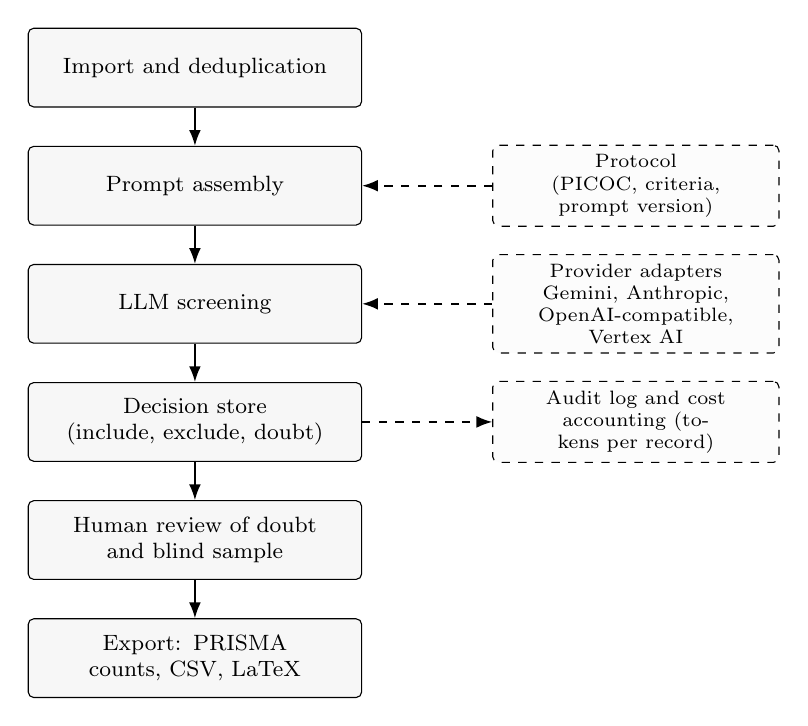
\begin{tikzpicture}[
  stage/.style={draw, rounded corners=2pt, align=center, font=\footnotesize,
                minimum height=10mm, text width=40mm, fill=black!3},
  side/.style={draw, dashed, rounded corners=2pt, align=center, font=\scriptsize,
               minimum height=10mm, text width=34mm, fill=black!1},
  arr/.style={-{Latex[length=2mm]}, semithick}
]
\node[stage] (s1) at (0,0) {Import and deduplication};
\node[stage] (s2) at (0,-1.5) {Prompt assembly};
\node[stage] (s3) at (0,-3.0) {LLM screening};
\node[stage] (s4) at (0,-4.5) {Decision store\\ (include, exclude, doubt)};
\node[stage] (s5) at (0,-6.0) {Human review of doubt and blind sample};
\node[stage] (s6) at (0,-7.5) {Export: PRISMA counts, CSV, LaTeX};

\node[side] (proto) at (5.6,-1.5) {Protocol\\ (PICOC, criteria, prompt version)};
\node[side] (prov)  at (5.6,-3.0) {Provider adapters\\ Gemini, Anthropic,\\ OpenAI-compatible, Vertex AI};
\node[side] (audit) at (5.6,-4.5) {Audit log and cost\\ accounting (tokens per record)};

\draw[arr] (s1) -- (s2);
\draw[arr] (s2) -- (s3);
\draw[arr] (s3) -- (s4);
\draw[arr] (s4) -- (s5);
\draw[arr] (s5) -- (s6);
\draw[arr, dashed] (proto) -- (s2);
\draw[arr, dashed] (prov) -- (s3);
\draw[arr, dashed] (s4) -- (audit);
\end{tikzpicture}
\caption{Path of a record through Sifter. Solid arrows are the screening
pipeline; dashed arrows are the components that make the pipeline
provider-independent and auditable.}
\label{fig:pipeline}
\end{figure}

Two implementation details are worth recording because they change the
interpretation of the results. First, screening is executed in batch: the
platform submits records in parallel and stores one event per state
transition, so the interval between consecutive events measures throughput,
not the time a reviewer would spend reading. Second, the \emph{doubt} label is
not an error state. It is the mechanism through which the model declines to
decide, and the queue gives those records priority over the ones the model
confidently excluded.

\subsection{Blind validation mode}\label{sec:blind}

The validation mode is the feature that distinguishes Sifter from a screening
interface with an API key. When a validation study is opened for a project,
the platform draws a random sample of records, hides the existing model
decision for those records in the reviewer interface, and asks the reviewer to
screen them without seeing the machine label. Only after the human decision is
stored does the interface reveal both decisions and update the statistics:
Cohen's $\kappa$ with a bootstrap confidence interval, raw agreement, the
confusion matrix and the derived sensitivity and specificity, computed against
the human decision as reference \autocite{Cohen_1960,Landis_1977}.

The sample, the seed used to draw it and the resulting pairs are stored, so
the study can be repeated on a different sample and compared with the earlier
one. This is the practical answer to the reproducibility requirement of the
journal's generative AI guidance \autocite{Farotimi_2025}: the agreement study
is an object inside the system, not a table typed into a manuscript.

\subsection{Critical appraisal with a weighted rubric}\label{sec:quality}

Screening decides what enters the corpus; it does not say how much each study
is worth. Sifter therefore has a second judgement stage, applied only to
included records, in which the reviewer scores each study against a quality
instrument defined in the protocol, following the practice of structured
appraisal tools for observational and experimental designs
\autocite{NOS_2000,CASP_2023}.

The instrument has two parts. The first is a list of criteria, each with a
weight. The second is a single answer scale shared by all criteria, whose
levels carry the degree of compliance (for example 4 for \emph{meets}, 3 for
\emph{partially meets}, down to 0 for \emph{fails}). Sharing one scale and
weighting the criteria, instead of writing a bespoke scale per criterion, keeps
the vocabulary stable across instruments and lets a criterion be promoted or
demoted without rewriting the instrument.

The score of a record is the weighted mean of the degrees of compliance, put
back on the scale of the instrument:

\begin{equation}
S = n \cdot \frac{\sum_{q=1}^{n} w_q\, s_q}{\sum_{q=1}^{n} w_q},
\qquad
S_{\max} = n \cdot \max_j v_j,
\label{eq:quality}
\end{equation}

where $n$ is the number of criteria, $w_q$ the weight of criterion $q$, $s_q$
the value of the answer recorded for it and $v_j$ the values of the answer
scale. The ceiling depends on the instrument the reviewer declared (two
criteria on a 0 to 4 scale give a maximum of 8) and not on the weights, which
only redistribute the requirement: with weights 2 and 1 the first criterion
accounts for two thirds of the score. The distinction matters because it keeps
the ceiling interpretable when a criterion is promoted; if weights inflated
the ceiling, one edit would change the meaning of every score already
recorded.

A study becomes eligible for extraction when $S$ reaches an acceptance cutoff.
The cutoff is stored in points, because other modules compare it with the score
in SQL, but its invariant is the percentage of the ceiling: when the ceiling
changes, the stored cutoff is recomputed to preserve the percentage the
reviewer chose, rather than the number of points.

\subsection{Changing an instrument with provenance}\label{sec:repricing}

Review protocols change, and a platform that forces the team to duplicate a
project to adjust a weight pushes the change outside the audit trail. Sifter
therefore allows the instrument to be edited after the first assessment, but
only as an operation with provenance. Once a vote exists the rubric is locked,
and saving a change requires an explicit confirmation that first shows the
effect: how many records are approved before and after, how many cross the
cutoff, and how many would drop to zero because an answer no longer exists in
the scale. On confirmation the server recomputes every derived score of the
project in one transaction, stores the previous instrument and the summary of
the impact in the project log, and exposes an undo that restores both. Each new
assessment stores the hash of the instrument it was produced under, so a score
can be traced to the version of the rubric that generated it, and the generated
report prints that version next to a note on any repricing.

Weights are the reviewer's methodological decision and are deliberately kept
out of the model prompt: the LLM can propose a score per criterion from the
criterion text, but never sees the weights, so that an important criterion is
not judged more leniently and a secondary one more severely. Criteria are free
text in the language of the project, so the same installation can host
instruments written in different languages.

\subsection{Export and reporting}

The platform exports the record set with both decisions, the audit events and
the counts needed for the PRISMA flow diagram: records identified, duplicates
removed, records screened, records excluded at screening and records sought for
retrieval \autocite{Page_2021}. The export includes the model identifier, the
protocol version and the prompt version for each decision, which is what makes
the screening stage auditable after publication.

\subsection{Implementation and availability}

Version 3.21.1 of the platform is written in Python and TypeScript and is
distributed as a Docker Compose stack. At the time of this revision the backend
suite contained 770 tests, of which 767 passed and three were skipped, with
81.27\% line coverage against a project gate of 33\%, and the frontend suite
contained 227 component tests. Source code, licence and installation
instructions are reported in the Data and Code Availability Statement.

\section{Pilot deployment}\label{sec:evaluation}

\subsection{Setting and data}

The numbers below come from the production database of a single installation
used by the first author between April and June 2026. They are a
\emph{deployment record}, not a controlled experiment: the projects were
screened because they had to be screened, not because they were designed as an
evaluation. We report them because they establish the order of magnitude of
cost and scale, and because the journal's guidance asks for exactly this kind
of operational evidence alongside the agreement study
\autocite{Farotimi_2025}. The formal agreement study on a fresh blind sample is
described in Section~\ref{sec:planned} and is not yet complete.

Four projects are included. Three of them are screening runs over the same
source of 4{,}670 records under different prompt configurations, which we
label P1, P2 and P3; the fourth, P4, is an educational corpus of 343 records
used to exercise the platform end to end.

\subsection{Scale and decision distribution}

Table~\ref{tab:corpus} summarises the corpus. Of 14{,}353 records, 14{,}219
(99.1\%) carry a stored model decision. The 134 records without one are
concentrated in P1, the earliest run, and correspond to records imported after
the batch had been executed. The proportion of records classified as
\emph{doubt} falls sharply across the three runs over the same source, from
176 in P1 to 27 in P3, which is consistent with successive prompt revisions
that pushed the model towards a binary decision.

\begin{table}[htbp]
\centering
\caption{Records, model decisions and decision distribution per project}
\label{tab:corpus}
\begin{tabular}{@{}lrrrrrrr@{}}
\toprule
Project & Records & With AI & Included & Excluded & Doubt & Duplicates & Inclusion \\
 & & decision & & & & & rate \\
\midrule
P1 & 4{,}670 & 4{,}573 (97.9\%) & 565 & 3{,}899 & 176 & 30 & 12.1\% \\
P2 & 4{,}670 & 4{,}652 (99.6\%) & 913 & 3{,}660 & 79 & 18 & 19.6\% \\
P3 & 4{,}670 & 4{,}651 (99.6\%) & 1{,}030 & 3{,}594 & 27 & 19 & 22.1\% \\
P4 & 343 & 343 (100\%) & 11 & 332 & 0 & 0 & 3.2\% \\
\midrule
Total & 14{,}353 & 14{,}219 (99.1\%) & 2{,}519 & 11{,}485 & 282 & 67 & 17.6\% \\
\bottomrule
\end{tabular}
\end{table}

The inclusion rate is the number that matters for planning, and it varies by a
factor of almost two across configurations of the same protocol (12.1\% in P1
against 22.1\% in P3). A review team that estimates reviewer workload from a
single automated run would therefore be wrong by a wide margin. This is an
argument for treating the automated decisions as a first pass whose yield has
to be measured per project, which is what the doubt mechanism and the blind
mode are for.

\subsection{Cost per record}

Table~\ref{tab:cost} reports token consumption. The aggregate is 11.85 million
tokens for 14{,}219 records, or 833 tokens per record, with a range from 427 to
1{,}149 depending on prompt length and abstract length. The three tariff
scenarios translate this into money; they span two orders of magnitude because
provider prices differ by that much, and the platform records the model per
decision so that the applicable tariff can be reconstructed later.

\begin{table}[htbp]
\centering
\caption{Token consumption per project (top) and the resulting cost of the
whole corpus under three provider tariffs (bottom). Tariffs are expressed in US
dollars per million input and output tokens}
\label{tab:cost}
\small
\begin{tabular}{@{}lrrr@{}}
\toprule
Project & Input tokens & Output tokens & Tokens per record \\
\midrule
P1 & 3{,}846{,}046 & 279{,}519 & 902 \\
P2 & 5{,}032{,}476 & 313{,}751 & 1{,}149 \\
P3 & 1{,}656{,}524 & 333{,}570 & 427 \\
P4 & 367{,}003 & 21{,}739 & 1{,}133 \\
\midrule
Total & 10{,}902{,}049 & 948{,}579 & 833 \\
\bottomrule
\end{tabular}

\vspace{2mm}
\begin{tabular}{@{}lrr@{}}
\toprule
Tariff (input / output) & Cost of the corpus & US\$ per 1{,}000 records \\
\midrule
Low (0.10 / 0.40) & US\$1.47 & 0.10 \\
Mid (0.30 / 2.50) & US\$5.64 & 0.40 \\
High (1.25 / 10.00) & US\$23.11 & 1.63 \\
\bottomrule
\end{tabular}
\end{table}

The order of magnitude is the finding: screening a 15{,}000-record review costs
between one and twenty-five US dollars in model calls. The binding constraint
on adoption is therefore not the price of inference but the reliability of the
decisions, which is what the next subsection addresses.

\subsection{Agreement with the human reviewer}

Table~\ref{tab:kappa} reports every pair of records for which both an
automated and a stored human decision existed at the time of measurement. We
report all four projects, including the two whose agreement is close to
chance, because suppressing them would reproduce the reporting practice the
guidance warns against \autocite{Farotimi_2025}.

\begin{table}[htbp]
\centering
\caption{Agreement between automated and stored human decisions, with the
confusion matrix of the four projects (VN, true negative; FP, false positive;
VP, true positive; FN, false negative)}
\label{tab:kappa}
\small
\begin{tabular}{@{}lrrrrl@{}}
\toprule
Project & Pairs & $\kappa$ & 95\% CI & Raw agreement & Confusion matrix \\
\midrule
P1 & 4 & 0.000 & not computed ($n<5$) & 50.0\% & 2 VN, 2 FP, 0 VP, 0 FN \\
P2 & 34 & 0.084 & 0.000 to 0.235 & 47.1\% & 14 VN, 18 FP, 2 VP, 0 FN \\
P3 & 34 & 0.013 & $-0.290$ to 0.294 & 47.1\% & 6 VN, 14 FP, 10 VP, 4 FN \\
P4 & 31 & 0.608 & 0.290 to 0.903 & 83.9\% & 20 VN, 5 FP, 6 VP, 0 FN \\
\bottomrule
\end{tabular}
\end{table}

Three observations follow, and the third is the one we consider most important.

First, only P4 supports an interpretation. With 31 pairs, $\kappa$ is 0.61
(95\% CI 0.29 to 0.90), raw agreement 83.9\%, sensitivity 100\% (six of six
included records recovered) and specificity 80\% (20 of 25 exclusions
confirmed). The interval is wide enough that the point estimate should not be
quoted as the accuracy of the tool; it is a signal, not a measurement.

Second, the error pattern in P2 and P3 is asymmetric and consistent across both
runs: over-inclusion, with 14 to 18 false positives against 0 to 4 false
negatives. In screening, a false negative costs evidence and a false positive
costs reviewer time. The configuration used in these runs is therefore
recall-oriented, which is defensible for a first pass but has a direct
consequence for workload: the reviewer still reads a substantial share of the
records, and the workload reduction is smaller than the raw automation rate
suggests.

Third, the low agreement in P2 and P3 is not evidence that the model cannot
screen. The stored human decisions in those projects were recorded during
development, at dates that were not captured, and may have been made under an
earlier version of the criteria. What the table demonstrates is a limitation of
the measurement, not of the model, and it is precisely the limitation that the
blind validation mode was built to remove: the platform now records who
decided, when, and against which protocol version, which the pilot data do not
carry for every pair.

\subsection{Engineering quality}

The platform's own test suite is reported because reproducibility of a
research tool is part of its evaluation. At the time of the pilot the backend
suite contained 260 tests, of which 259 passed and one was skipped, in 2
minutes and 42 seconds, with 75.11\% line coverage. Throughput during batch
execution produced a median interval between consecutive decision events of
0.00 to 0.05 seconds per project, confirming that screening runs in a single
batch rather than interactively; it is not a measure of reviewer time.

\subsection{What has not been measured}\label{sec:planned}

The guidance for generative AI submissions requires workload metrics for tools
whose purpose is to reduce effort \autocite{Farotimi_2025}. Sifter has not yet
produced them, and we state the gap rather than approximate it. Three
quantities are outstanding.

\begin{enumerate}
\item \textbf{Work saved over screening (WSS)} and \textbf{number needed to
read (NNR)}, computed on a blind sample of 300 pairs drawn from the
educational corpus. The sample and the reference decisions have been generated
and are stored; the reference screening has not been completed.
\item \textbf{Reviewer time per record}, with and without the automated first
pass, which requires a timed screening session and is the input for any
statement about hours saved.
\item \textbf{External validation} on a review protocol and record set produced
by another team, which is the only way to test transfer across fields and
prompt styles.
\end{enumerate}

Until these three exist, the claim this paper supports is bounded: the
platform records what it does, at a cost that is negligible relative to
reviewer time, and it makes the agreement study cheap enough to be run as
routine quality control. It does not yet support a claim about accuracy in
general.

\section{Discussion}\label{sec:discussion}

\subsection{What the pilot establishes}

Three things, in decreasing order of confidence. The cost of screening a
record with a general-purpose model is between US\$0.0001 and US\$0.0016 at
current tariffs, which is small enough that the price of inference cannot be
the reason a review team declines to automate the first pass. The platform can
hold and audit a screening run of several thousand records with per-record
provenance, which the pilot exercised four times. And the agreement between
model and reviewer can be computed by the tool itself, which changes the
economics of validation: an agreement study stops being a separate research
project and becomes a button in the project dashboard.

\subsection{Error asymmetry is the design problem, not accuracy}

The pilot's most transferable observation is the shape of the errors, not their
rate. Across the two runs that produced interpretable matrices, false positives
outnumbered false negatives by roughly five to one. For a first-pass screen
this is the correct direction to err in, and it is also the reason why
reporting a single ``accuracy'' number for a screening tool is uninformative:
the same model can be tuned to miss nothing and to save little, or to save a
great deal and to miss studies. Sifter exposes the choice instead of concealing
it, through the three-way decision space and through the doubt queue, which
prioritises precisely the records on which the model declined to commit.

Whether the recall-oriented configuration is the right default for evidence
synthesis is an empirical question that this paper does not answer, and that
the field has not answered either. What the platform contributes is the
ability to state the configuration, measure its consequence and change it
without rewriting the tool.

\subsection{Provider independence as a methodological requirement}

Model behaviour changes with versions, prompts and sampling temperature, and
the guidance for generative AI submissions now requires the model version and
access date to be recorded \autocite{Farotimi_2025}. A tool that hard-codes one
provider cannot honour that requirement across a multi-year review, because
the model it used in the first year may not exist in the second. Sifter
therefore separates the protocol, the prompt template and the provider, and
stores the triplet with each decision. This is an engineering decision with a
methodological justification: it is what allows a review published in 2026 to
be re-screened in 2029 with the same protocol and a different model, and the
difference attributed to the model rather than to the protocol.

\subsection{Reporting against the guidance}

Table~\ref{tab:guidance} maps the journal's requirements for manuscripts
evaluating generative AI \autocite{Farotimi_2025} to the sections of this
paper. The last row is the honest one.

\begin{table}[htbp]
\centering
\caption{Reporting requirements for generative AI evaluations and where each is
addressed}
\label{tab:guidance}
\begin{tabular}{@{}p{0.34\textwidth}p{0.56\textwidth}@{}}
\toprule
Requirement & Where addressed \\
\midrule
Sampling and dataset characteristics &
Section~\ref{sec:evaluation}, Table~\ref{tab:corpus}; the 300-pair blind sample
is described in Section~\ref{sec:planned} \\
Prompt development and testing &
Section~\ref{sec:protocol}; prompts are versioned with the protocol \\
Established performance metrics &
Agreement, sensitivity and specificity in Table~\ref{tab:kappa}; WSS and NNR
outstanding \\
Benchmark against manual screening &
Table~\ref{tab:kappa}, with the provenance limitation stated \\
Quality assurance procedures &
Blind validation mode, Section~\ref{sec:blind} \\
Seeds and randomisation &
Sample selection is seeded and stored with the validation study \\
Computational environment and model versions &
Section~\ref{sec:system} and the per-decision record; versions and access dates
in the Data and Code Availability Statement \\
External validation &
Outstanding; Section~\ref{sec:planned} \\
\bottomrule
\end{tabular}
\end{table}

\subsection{Limitations}

The pilot has four limitations that a reader should carry into any use of the
numbers. It is a single installation used by a single reviewer, so
between-reviewer variability is not represented. The stored human decisions
were not made under a uniform protocol version and their timestamps were not
captured for every pair, which is why only one project yields an interpretable
$\kappa$. The evaluation covers title and abstract screening only; full-text
screening, the critical-appraisal stage described in
Section~\ref{sec:quality} and data extraction are outside the scope of this
paper, although the platform implements both later stages. And the reference
standard in the agreement study is one human reviewer, not consensus between
two, which means the reported agreement is a lower bound on agreement with a
methodologically correct reference.

\subsection{Implications for practice}

For a review team, the practical implication is a change in what has to be
planned. The automated first pass does not remove the need for screening; it
changes the object that has to be validated. Instead of asserting that a tool
was used, the team can report how many records the tool screened, with which
model and prompt, at what cost, and with what agreement against a blind human
sample. Review protocols and PRISMA flow diagrams already have slots for part
of this information; the rest would need a reporting convention, and the
guidance cited above is a first step towards one.

For tool builders, the implication is that the unit of contribution is not the
prompt but the audit trail. A prompt that screens well on a benchmark and
leaves no record of what it saw is not reusable in evidence synthesis, however
good its numbers are.

\section{Conclusion}\label{sec:conclusion}

Sifter is an open-source platform for large language model assisted screening
in systematic reviews, built around the proposition that an automated decision
is only useful to evidence synthesis when it is auditable, attributable to a
protocol and a model version, priced per record and measurable against a human
reviewer. The pilot deployment reported here screened 14{,}219 records at 833
tokens per record, at a monetary cost that is small against the reviewer time it
displaces, and produced an agreement estimate of
$\kappa = 0.61$ on the one corpus where the comparison was interpretable, with
no missed inclusions in a sample of 31 records. Those numbers are a signal, not
a validation: work saved over screening, number needed to read, reviewer time
and external validation remain to be measured, and the platform is instrumented
to measure them.

The broader claim is methodological rather than technical. As language models
become routine in screening, the scarce resource stops being inference and
becomes the evidence that the screening was done as reported. A tool that
records the model, the prompt, the protocol version, the cost and the human
comparison for every record makes that evidence a by-product of the work rather
than a separate publication.

\section*{Acknowledgements}

%% TODO: agradecimentos (bolsa, programa, revisores).

\section*{Data and Code Availability Statement}

%% TODO antes da submissao:
%% - repositorio publico do codigo, com LICENSE OSI (hoje o repositorio nao tem licenca);
%% - DOI do arquivo de dados (Zenodo ou OSF) com o corpus de medicao anonimizado;
%% - versao do modelo, data de acesso e prompt versionado de cada projeto do piloto;
%% - semente usada no sorteio da amostra cega de 300 pares.
The platform source code is available at \url{https://github.com/fgscaglioni/sifter-ai}.
The measurement corpus, the prompt versions and the seeded blind sample that
support Tables~\ref{tab:corpus} to~\ref{tab:kappa} are archived at
\emph{[repository DOI to be inserted before submission]}.
Model identifiers, versions and access dates are recorded per decision in the
archived dataset.

\section*{Funding Statement}

This research received no specific grant from any funding agency, commercial or
not-for-profit sectors.

\section*{Competing Interests}

The author declares none.

\section*{Author Contributions}

F.G.S. conceptualised the platform, wrote the software, designed and ran the
pilot, and wrote the manuscript.

\section*{Use of Artificial Intelligence Tools}

%% TODO: declarar aqui, conforme a politica da CUP, o uso de ferramentas de IA na
%% redacao do manuscrito (geracao de texto, traducao, revisao de linguagem) e
%% distinguir esse uso do objeto de estudo, que sao os LLMs usados pelo Sifter.


\begin{Backmatter}
\printbibliography
\end{Backmatter}

\end{document}
